\documentclass{standalone}
\usepackage{tikz}
\usepackage{pgfplots}

\begin{document}

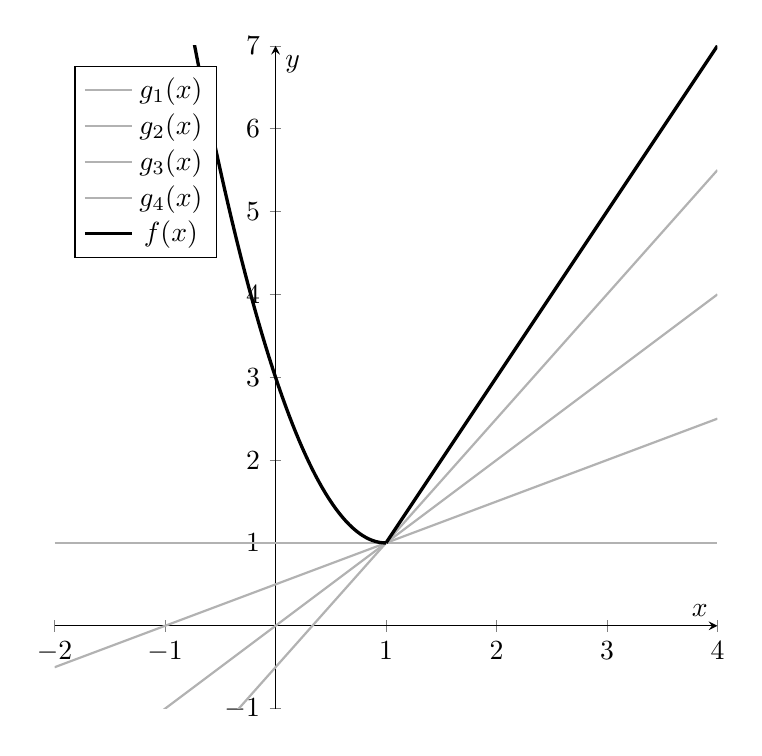
\begin{tikzpicture}
    \begin{axis}[
            axis lines = middle,
            xlabel = $x$,
            ylabel = $y$,
            xmin = -2, xmax = 4,
            ymin = -1, ymax = 7,
            xtick = {-2,-1,0,1,2,3,4},
            ytick = {-1,0,1,2,3,4,5,6,7},
            legend pos = north west,
            width = 10cm,
            height = 10cm,
            axis line style={-stealth},
        ]

        \addplot[domain=-2:4, gray!60, thick] {0*(x-1) + 1};
        \addplot[domain=-2:4, gray!60, thick] {1.5*(x-1) + 1};
        \addplot[domain=-2:4, gray!60, thick] {0.5*(x-1) + 1};
        \addplot[domain=-2:4, gray!60, thick] {(x-1) + 1};

        \addplot[domain=-2:1, black, very thick, samples=100] {2*(x-1)^2 + 1};
        \addplot[domain=1:4, black, very thick, samples=100] {2*(x-1) + 1};

        \legend{$g_1(x)$, $g_2(x)$, $g_3(x)$, $g_4(x)$, $f(x)$}
    \end{axis}
\end{tikzpicture}

\end{document}